\documentclass{article}
\usepackage{graphicx}
\usepackage{graphics}
\graphicspath{{/home/user/images/},{/home/personnels/berhe/TextClassification/}}
\usepackage{amsmath}
\usepackage{fancyhdr}

\setlength{\parindent}{0em}
\setlength{\parskip}{1em}
\renewcommand{\baselinestretch}{1.5}

\pagestyle{fancy}
\fancyhf{}
\rfoot{Page \thepage}
\lfoot{text classification}

\title{Text Classification }
\author{Aman Berhe}

\begin{document}
\maketitle
\newpage

\section{Tf-Idf}

To compute the tf-idf i have used the two documents and the frequency of the terms. Since we only have two documents and the terms can be found either in one or in both of the documents, Simplifying the computation of the log i have done the following

if the term exist in both of the documents: put 0

		since $\log(2/2)$ is $0$
		
else multiply the frequency by $0.3$

		since $\log(2/1)$ is $0.301029996$
		
here are the results and plot
\subsection{Tf-Idf for positive}
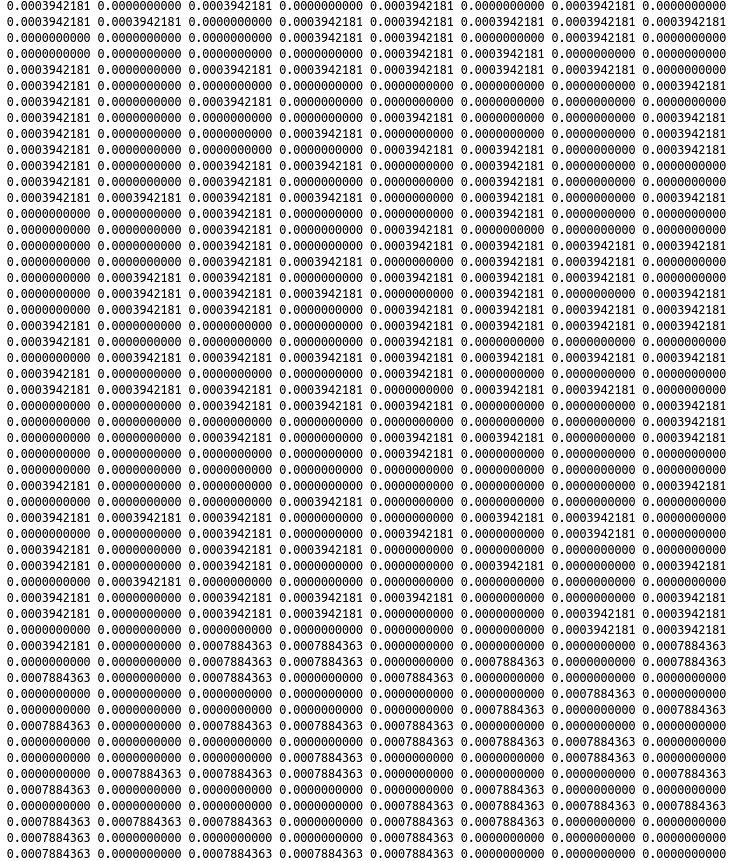
\includegraphics[width=0.8\linewidth]{tf_idf_pos1.png}\\
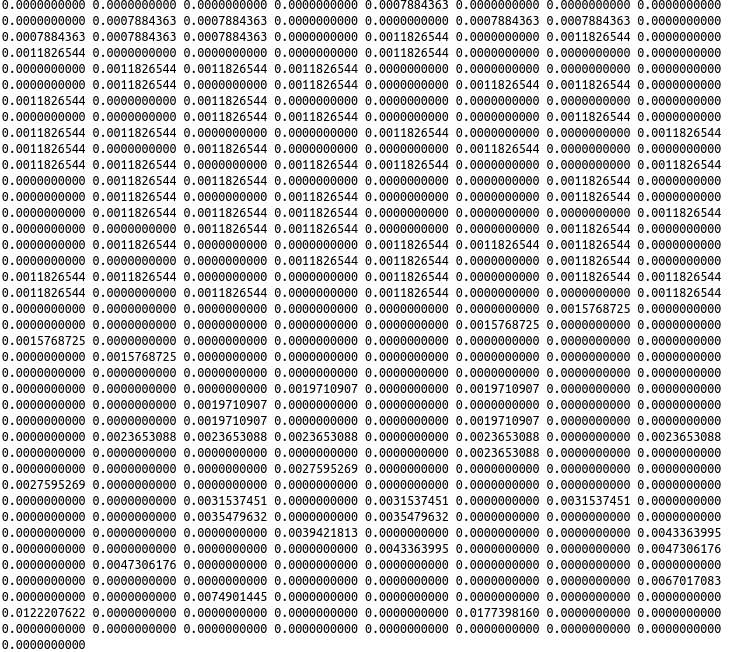
\includegraphics[width=0.8\linewidth]{tf_idf_pos2.png}\\
the Plot looks like this

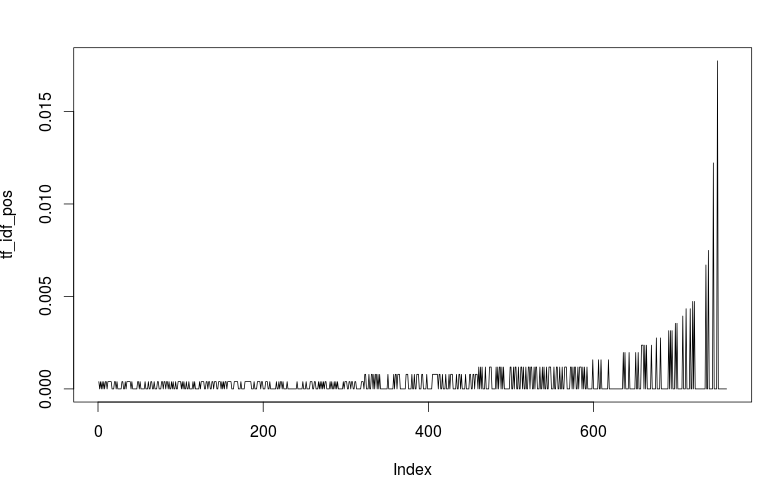
\includegraphics[width=0.8\linewidth]{tf_idf_pos3.png}
\subsection{Tf-Idf for positive with the number of sentences}

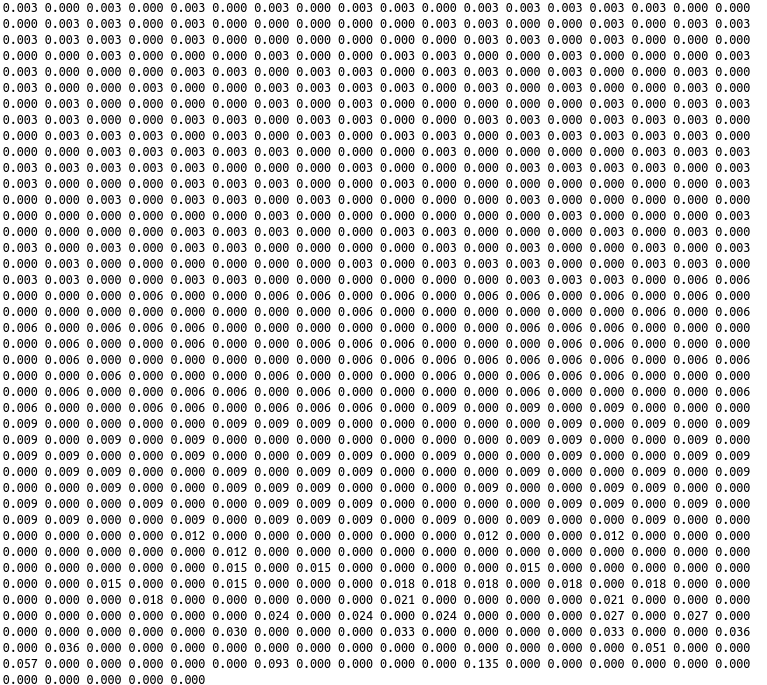
\includegraphics[width=0.8\linewidth]{tf_idf_posusingsentence.png}\\
the Plot looks like this

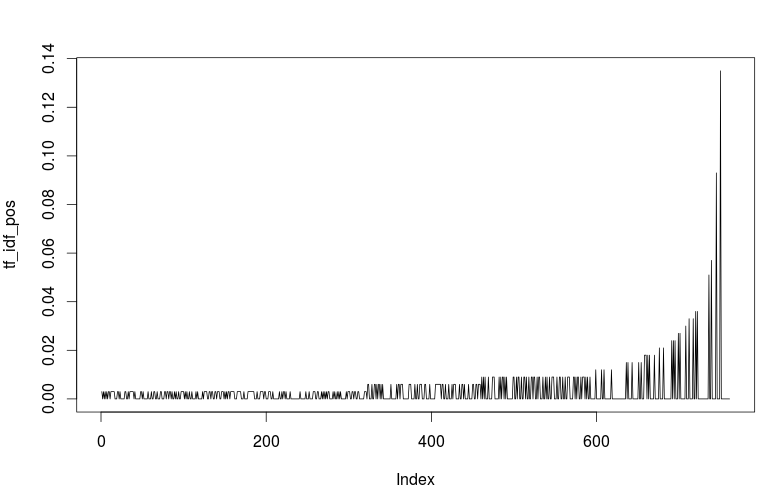
\includegraphics[width=0.8\linewidth]{tf_idf_posusingsentenceplot.png}\\

\subsection{Tf-Idf for negative}
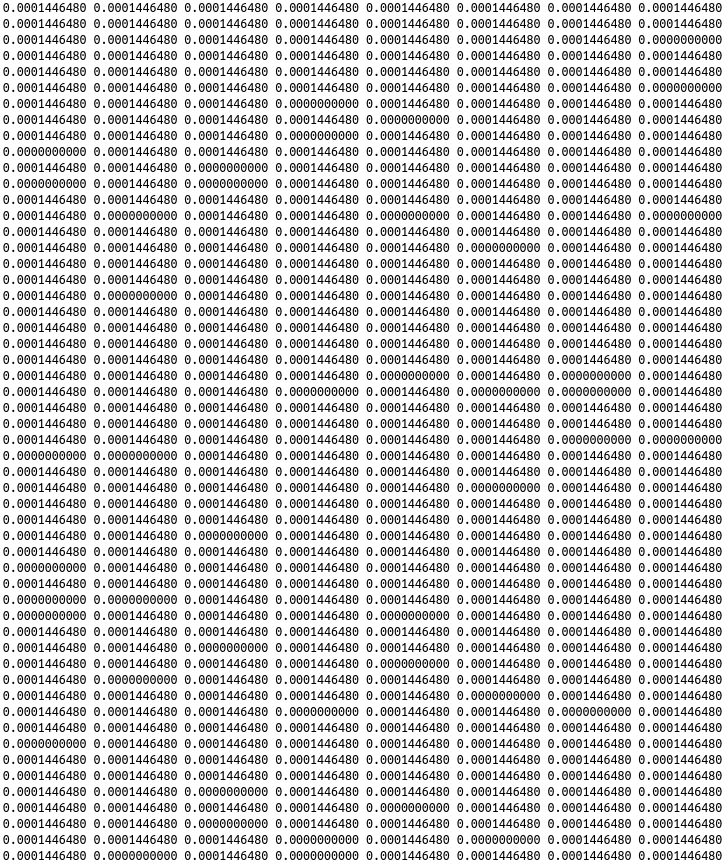
\includegraphics[width=0.8\linewidth]{tf_idf_neg1.png}\\
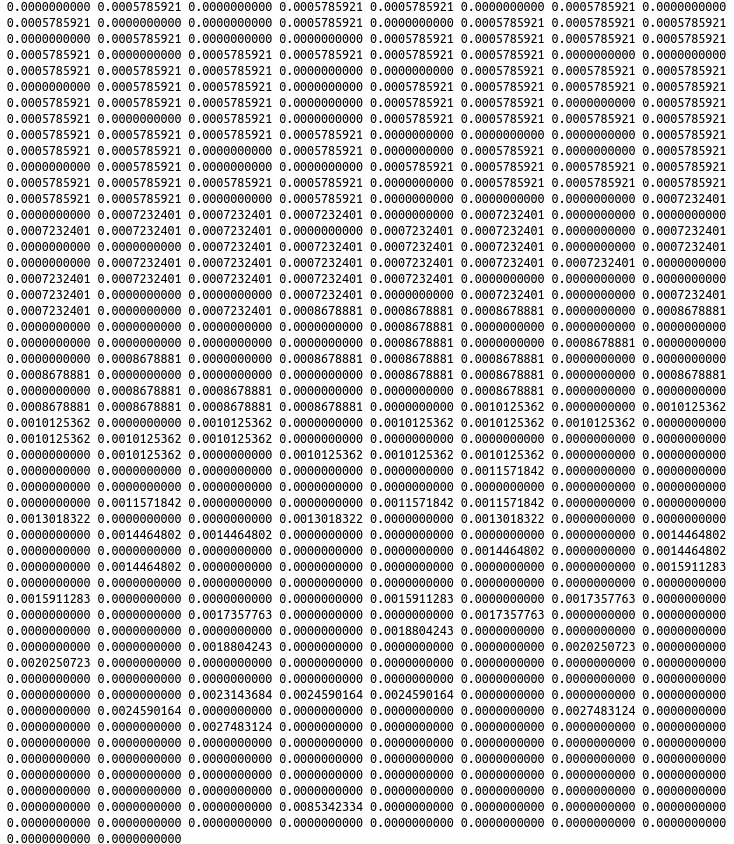
\includegraphics[width=0.8\linewidth]{tf_idf_neg2.png}\\
the Plot looks like this

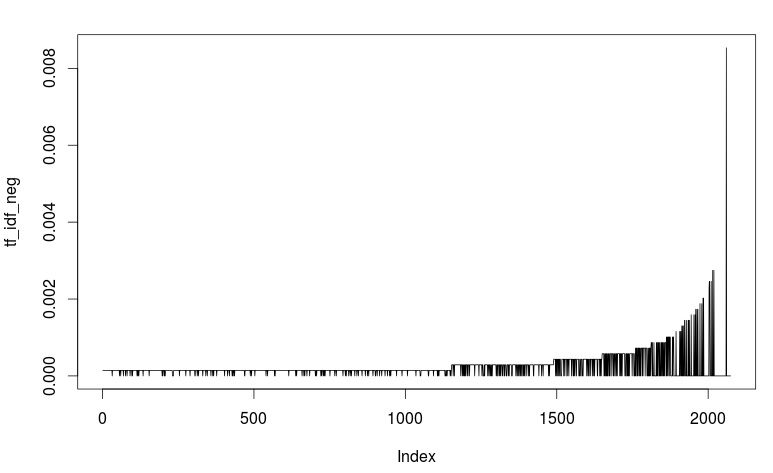
\includegraphics[width=0.8\linewidth]{tf_idf_neg3.png}
\subsection{Tf-Idf for negative with the number of sentences}

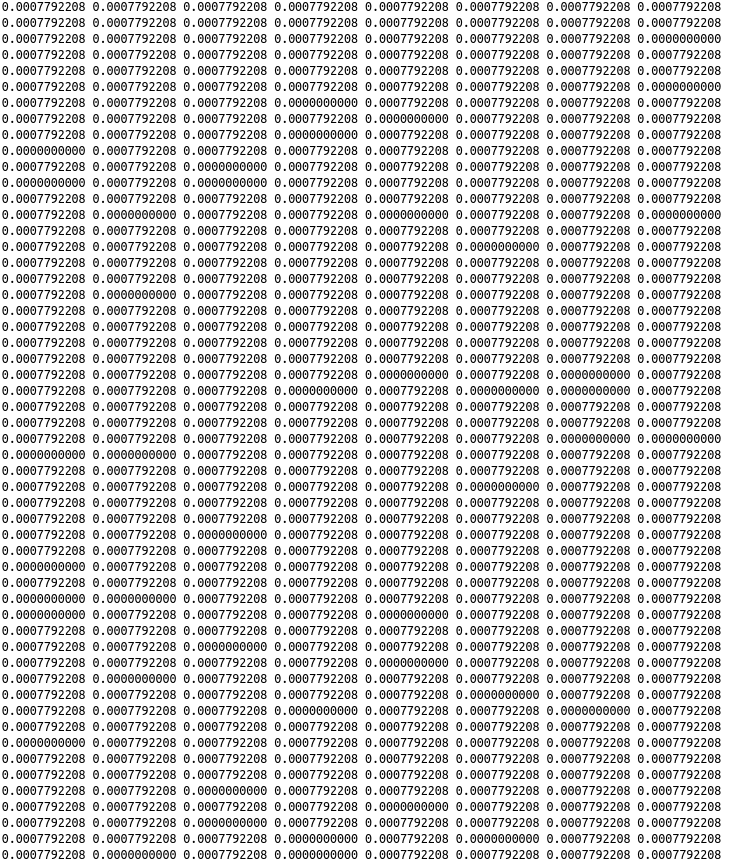
\includegraphics[width=0.8\linewidth]{tf_idf_neg_usingsentence1.png}\\
the Plot looks like this

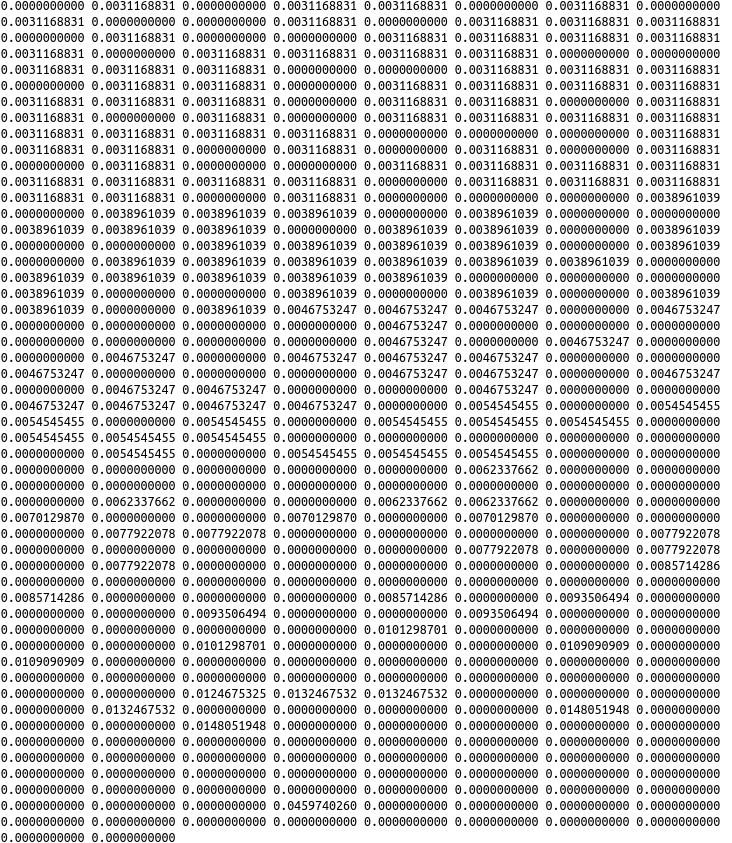
\includegraphics[width=0.8\linewidth]{tf_idf_neg_usingsentence2.png}
\end{document}